%%----------------------------------------------------------------------------
%% Presentatie HoGent Bedrijf en Organisatie
%%----------------------------------------------------------------------------
%% Auteur: Bert Van Vreckem [bert.vanvreckem@hogent.be]

\documentclass{beamer}

%==============================================================================
% Aanloop
%==============================================================================

%---------- Packages ----------------------------------------------------------

\usepackage{graphicx,multicol}
\usepackage{comment,enumerate,hyperref}
\usepackage{amsmath,amsfonts,amssymb}
\usepackage{tikz}
\usepackage[dutch]{babel}
\usepackage[utf8]{inputenc}
\usepackage{multirow}
\usepackage{eurosym}
\usepackage{listings}
\usepackage[T1]{fontenc}
\usepackage{lmodern}
\usepackage{textcomp}
\usepackage{framed}
\usepackage{wrapfig}

%---------- Configuratie ------------------------------------------------------

\usetikzlibrary{arrows,shapes,backgrounds,positioning,shadows}

\usetheme{hogent}

%---------- Commando-definities -----------------------------------------------

\newcommand{\tabitem}{~~\llap{\textbullet}~~}

%---------- Info over de presentatie ------------------------------------------

\title[Intro]{Coding For Dummies}
\author{Jens {Buysse}}
\date{\today}

%==============================================================================
% Inhoud presentatie
%==============================================================================

\begin{document}

%---------- Front matter ------------------------------------------------------

% Dia met het HoGent logo
\HoGentLogo

% Titeldia met faculteitslogo
\titleframe

%---------- Inhoud ------------------------------------------------------------

\begin{frame}
  \frametitle{Inhoud}

  \tableofcontents
\end{frame}

\section{De eerste codes}

\begin{frame}{Cryptografie}
	Het woord \textcolor{HoGentBlue}{cryptografie} betekent letterlijk  \textcolor{HoGentBlue}{‘geheim schrijven’} of  \textcolor{HoGentBlue}{‘verborgen schrijven’}, het is voortgekomen uit de 2 griekse woorden 
	\begin{itemize}
		\item kruptos en
		\item graphein
	\end{itemize}
	 wat samen ‘geheim schrijven’ betekent.
\end{frame}

\begin{frame}{De eerste codes}
	Zowel de Romeinen als de Grieken verdiepten zich in de grondbeginselen van cryptografie. 
	
	\begin{itemize}
		\item Optische signalen m.b.h.v. toortsen
		\item vlaggen
		\item spiegels
		\item \dots
	\end{itemize}
\end{frame}

\begin{frame}{De eerste codes}
	\begin{figure}
		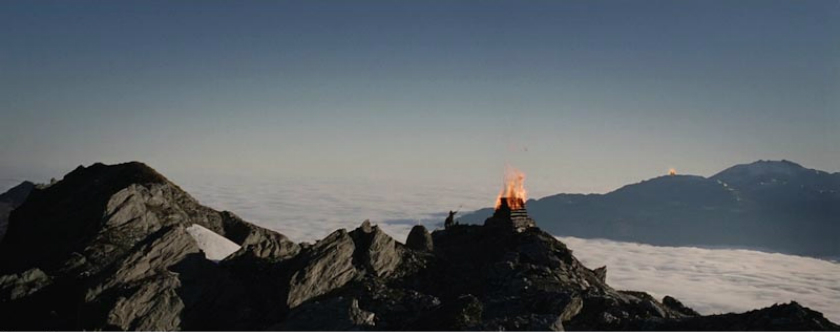
\includegraphics[width=\textwidth]{img/toorts.jpg}
	\end{figure}
\end{frame}

\begin{frame}{Polybius}
	Code ontwikkeld door Griekse militair.
	\[ \begin{bmatrix}
		& 1  & 2  & 3  & 4 & 5\\ 
		1 & A  & B  &  C & D & E\\ 
		2 & F & G  & H  & I  & J \\ 
		3 & K & L  & M  & N  & O \\ 
		4 & P & Q & R & S  &  T\\ 
		5 & V & W & X & Y & Z  
	\end{bmatrix}  \]
	Wat betekent volgend geheimschrift?
	\[ \begin{bmatrix}
12 & 53 & 34 & 54 & 15 & 43 & 51 & 12 & 11 & 15 \\ 
53 & 34 & 44 & 54 & 32 & 51 & 21 & 53 &23 &41 
\end{bmatrix} \]
\end{frame}

\begin{frame}{Polybius}
	Er werden twee reeksen van fakkels opgesteld:
	\begin{enumerate}
		\item Eerste 5 fakkels duiden de rij aan
		\item Tweede 5 fakkels duiden de kolom aan
	\end{enumerate}
\end{frame}

\begin{frame}{Aenas' Telegraaf}
		\begin{figure}
		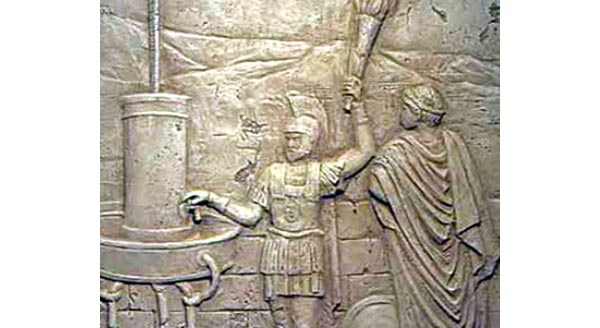
\includegraphics[width=\textwidth]{img/aenas.jpg}
	\end{figure}
\end{frame}

\begin{frame}{Aenas' Telegraaf}
	\begin{enumerate}
		\item Partij A heft een brandende fakkel
		\item Partij B heft ten antwoord ook een brandende fakkel
		\item Partij A laat fakkel zaken en kranen worden open gezet
		\item Partij A heft opnieuw brandende fakkel op zodat kranen gesloten kunnen worden.
	\end{enumerate}
\end{frame}

\begin{frame}[fragile]{Caesarscode}
	Elke letter wordt vervangen door de letter die een afgesproken aantal plaatsen (bv. 3) verder in het alfabet staat. 
	

	\begin{block}{Code}
	EDG LV D SODQ ZKLFK FDQQRW EHDU D FKDQJH
	\end{block}

\end{frame}

\begin{frame}[fragile]{Caesarscode - zwaktes}
	Wat zijn de zwaktes van deze codering en hoe zou je deze aanpakken?
	\pause
	\begin{itemize}
		\item Biedt slechts 25 mogelijkheden tot versleuteling. (Computer kan dit makkelijk kraken)
		\item De letter E komt heel erg vaak voor in de taal. Door te tellen welke letter het meest voorkomt kan je al goed raden wat de E zal zijn. 
		\item Je weet ook al wat de woorden zijn.
	\end{itemize}

\begin{center}
	\begin{block}{Code}
ROHXD VDBCK ANJTC QNUJF MXRCC XBNRI
NYXFN ARWJU UXCQN ALJBN BXKBN AENRC
\end{block}
\end{center}
\end{frame}

\begin{frame}[fragile]{Scytale}
	\begin{figure}
		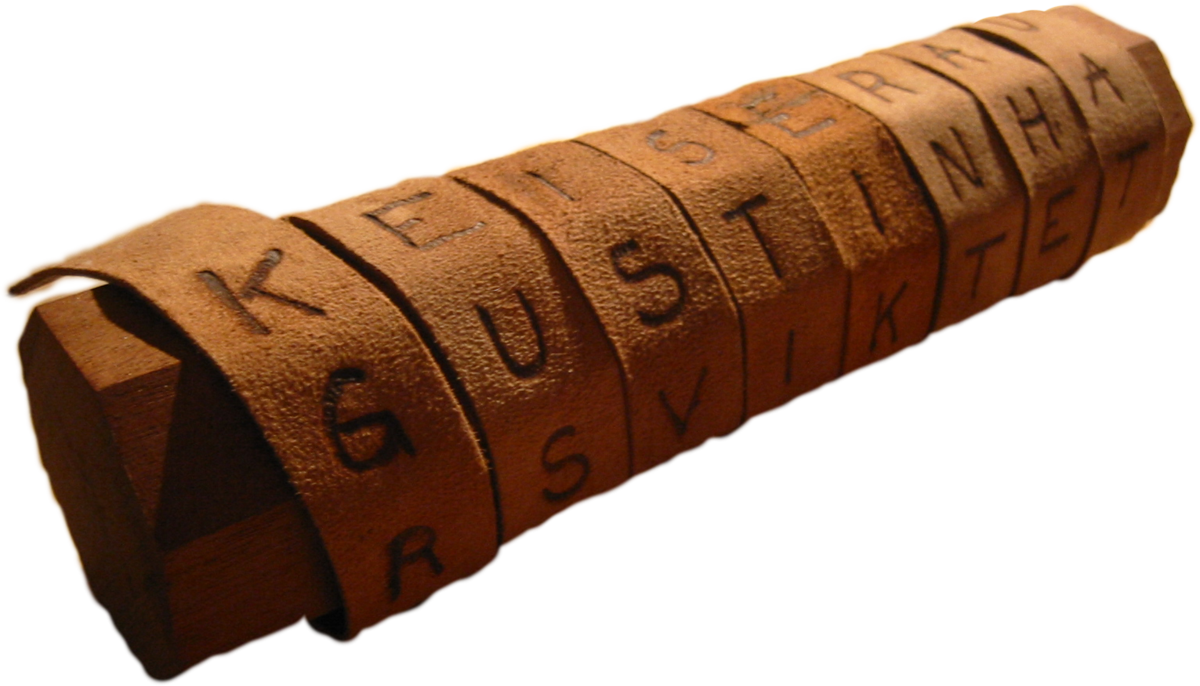
\includegraphics[width=\textwidth]{img/scytale}
	\end{figure}

\begin{block}{Code}
	ANACD DEIOR SUTWB AOTIR FNSUE ELNTF EHRMA IYNE
\end{block}

\end{frame}

\section{Iets formeler}

\begin{frame}{Adam, Alice \& Eve}
	\begin{figure}
		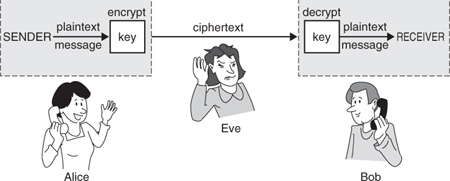
\includegraphics[width=\textwidth]{img/adameve.jpg}
	\end{figure}
\end{frame}

\begin{frame}{Cryptografieindeling}
	\begin{description}
		\item[Symmetrisch] Wanneer de sleutel om te versleutelen en ontsleutelen dezelfde is. Versleuteling kan enkel veilig gebeuren wanneer er een veilige sleuteluitwisseling tussen Alice en Bob gebeurd is.
	\item[Assymetrisch] Of ook publieke sleutel cryptografie waarbij het versleutelen en ontsleutelen met een verschillende sleutel moet. 
\end{description}
We merken op dat hedendaagse versleutelingsmechanismen vaak geen gelaagde combinatie van bovengenoemde types zijn.
\end{frame}

%---------- Back matter -------------------------------------------------------

\end{document}
